\documentclass[1p]{elsarticle_modified}
%\bibliographystyle{elsarticle-num}

%\usepackage[colorlinks]{hyperref}
%\usepackage{abbrmath_seonhwa} %\Abb, \Ascr, \Acal ,\Abf, \Afrak
\usepackage{amsfonts}
\usepackage{amssymb}
\usepackage{amsmath}
\usepackage{amsthm}
\usepackage{scalefnt}
\usepackage{amsbsy}
\usepackage{kotex}
\usepackage{caption}
\usepackage{subfig}
\usepackage{color}
\usepackage{graphicx}
\usepackage{xcolor} %% white, black, red, green, blue, cyan, magenta, yellow
\usepackage{float}
\usepackage{setspace}
\usepackage{hyperref}

\usepackage{tikz}
\usetikzlibrary{arrows}

\usepackage{multirow}
\usepackage{array} % fixed length table
\usepackage{hhline}

%%%%%%%%%%%%%%%%%%%%%
\makeatletter
\renewcommand*\env@matrix[1][\arraystretch]{%
	\edef\arraystretch{#1}%
	\hskip -\arraycolsep
	\let\@ifnextchar\new@ifnextchar
	\array{*\c@MaxMatrixCols c}}
\makeatother %https://tex.stackexchange.com/questions/14071/how-can-i-increase-the-line-spacing-in-a-matrix
%%%%%%%%%%%%%%%

\usepackage[normalem]{ulem}

\newcommand{\msout}[1]{\ifmmode\text{\sout{\ensuremath{#1}}}\else\sout{#1}\fi}
%SOURCE: \msout is \stkout macro in https://tex.stackexchange.com/questions/20609/strikeout-in-math-mode

\newcommand{\cancel}[1]{
	\ifmmode
	{\color{red}\msout{#1}}
	\else
	{\color{red}\sout{#1}}
	\fi
}

\newcommand{\add}[1]{
	{\color{blue}\uwave{#1}}
}

\newcommand{\replace}[2]{
	\ifmmode
	{\color{red}\msout{#1}}{\color{blue}\uwave{#2}}
	\else
	{\color{red}\sout{#1}}{\color{blue}\uwave{#2}}
	\fi
}

\newcommand{\Sol}{\mathcal{S}} %segment
\newcommand{\D}{D} %diagram
\newcommand{\A}{\mathcal{A}} %arc


%%%%%%%%%%%%%%%%%%%%%%%%%%%%%5 test

\def\sl{\operatorname{\textup{SL}}(2,\Cbb)}
\def\psl{\operatorname{\textup{PSL}}(2,\Cbb)}
\def\quan{\mkern 1mu \triangleright \mkern 1mu}

\theoremstyle{definition}
\newtheorem{thm}{Theorem}[section]
\newtheorem{prop}[thm]{Proposition}
\newtheorem{lem}[thm]{Lemma}
\newtheorem{ques}[thm]{Question}
\newtheorem{cor}[thm]{Corollary}
\newtheorem{defn}[thm]{Definition}
\newtheorem{exam}[thm]{Example}
\newtheorem{rmk}[thm]{Remark}
\newtheorem{alg}[thm]{Algorithm}

\newcommand{\I}{\sqrt{-1}}
\begin{document}

%\begin{frontmatter}
%
%\title{Boundary parabolic representations of knots up to 8 crossings}
%
%%% Group authors per affiliation:
%\author{Yunhi Cho} 
%\address{Department of Mathematics, University of Seoul, Seoul, Korea}
%\ead{yhcho@uos.ac.kr}
%
%
%\author{Seonhwa Kim} %\fnref{s_kim}}
%\address{Center for Geometry and Physics, Institute for Basic Science, Pohang, 37673, Korea}
%\ead{ryeona17@ibs.re.kr}
%
%\author{Hyuk Kim}
%\address{Department of Mathematical Sciences, Seoul National University, Seoul 08826, Korea}
%\ead{hyukkim@snu.ac.kr}
%
%\author{Seokbeom Yoon}
%\address{Department of Mathematical Sciences, Seoul National University, Seoul, 08826,  Korea}
%\ead{sbyoon15@snu.ac.kr}
%
%\begin{abstract}
%We find all boundary parabolic representation of knots up to 8 crossings.
%
%\end{abstract}
%\begin{keyword}
%    \MSC[2010] 57M25 
%\end{keyword}
%
%\end{frontmatter}

%\linenumbers
%\tableofcontents
%
\newcommand\colored[1]{\textcolor{white}{\rule[-0.35ex]{0.8em}{1.4ex}}\kern-0.8em\color{red} #1}%
%\newcommand\colored[1]{\textcolor{white}{ #1}\kern-2.17ex	\textcolor{white}{ #1}\kern-1.81ex	\textcolor{white}{ #1}\kern-2.15ex\color{red}#1	}

{\Large $\underline{12a_{0675}~(K12a_{0675})}$}

\setlength{\tabcolsep}{10pt}
\renewcommand{\arraystretch}{1.6}
\vspace{1cm}\begin{tabular}{m{100pt}>{\centering\arraybackslash}m{274pt}}
\multirow{5}{120pt}{
	\centering
	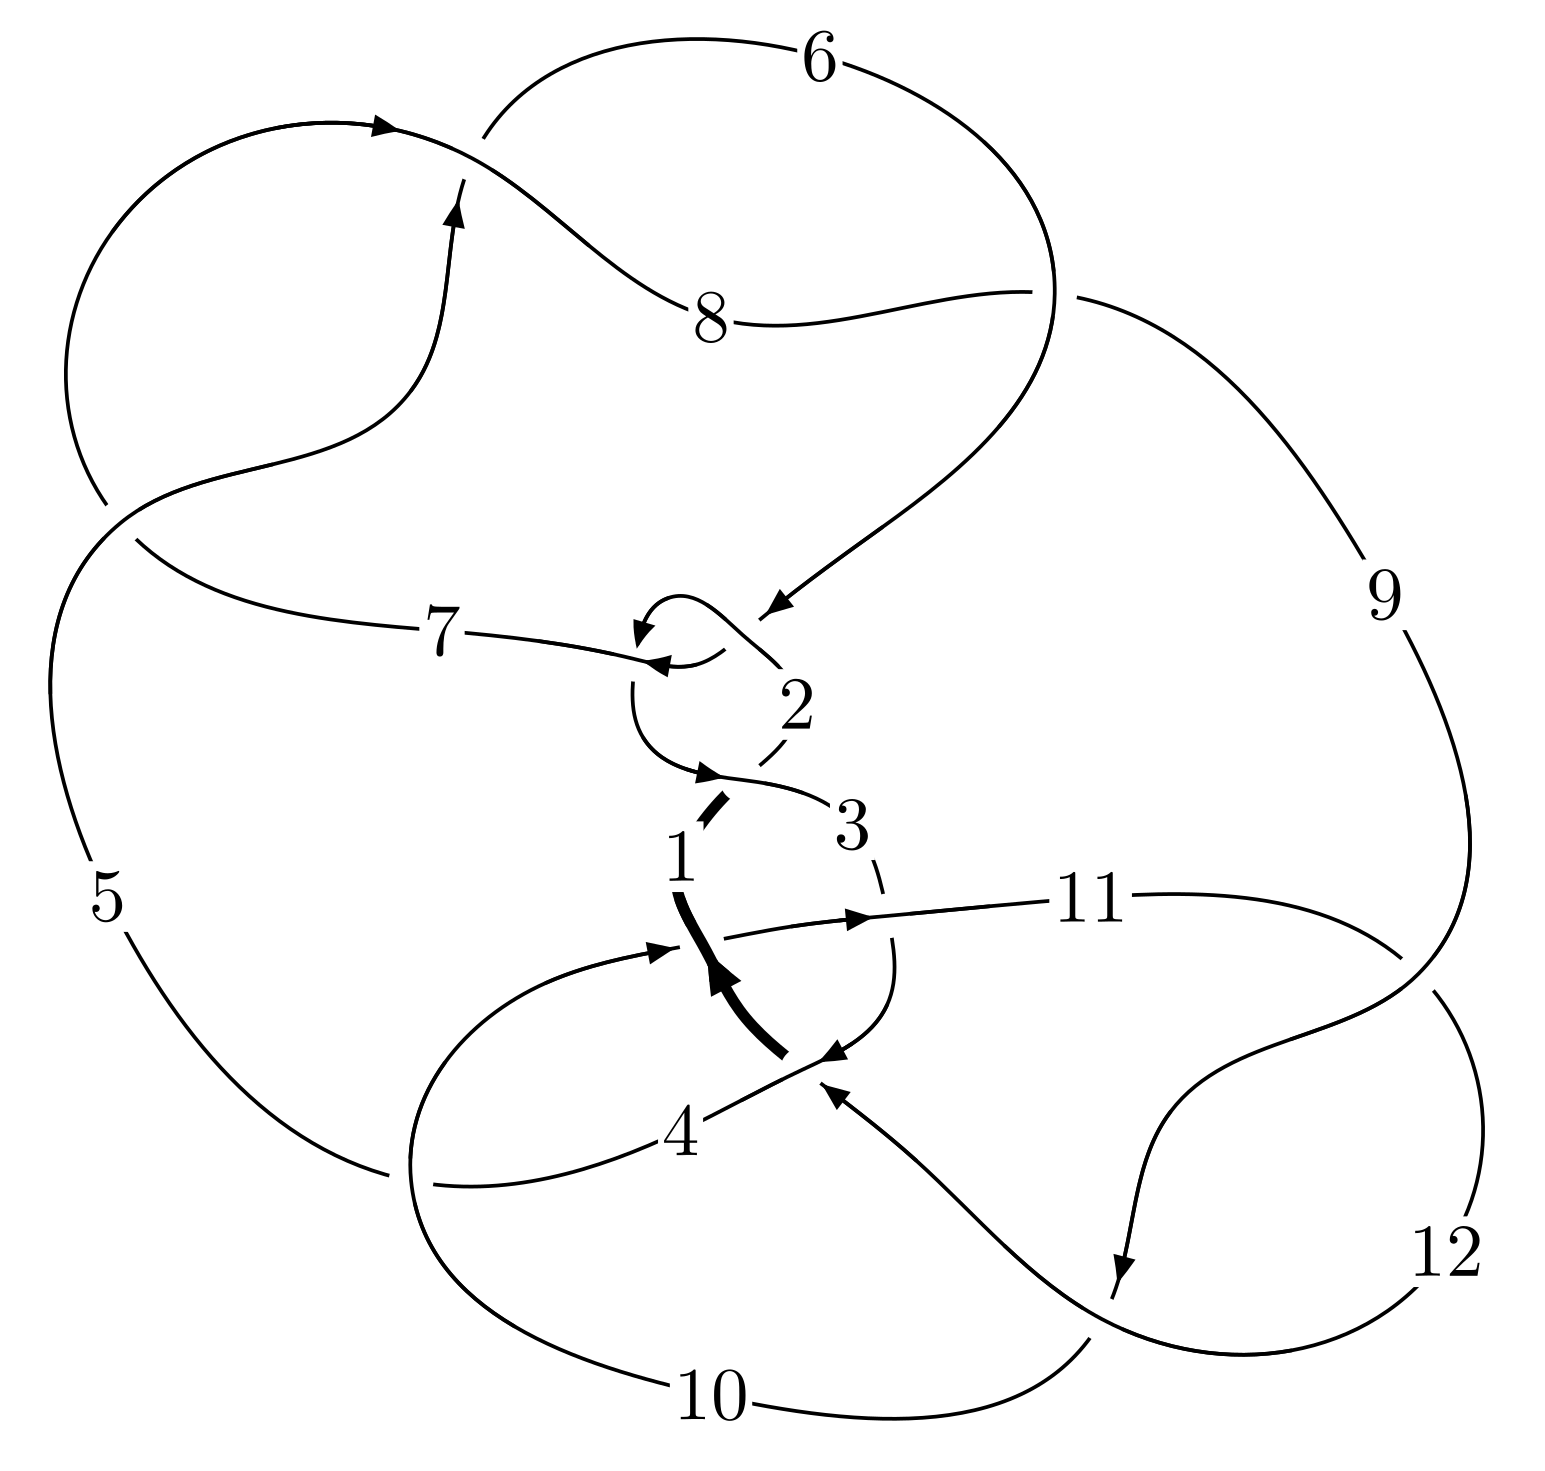
\includegraphics[width=112pt]{../../../GIT/diagram.site/Diagrams/png/1476_12a_0675.png}\\
\ \ \ A knot diagram\footnotemark}&
\allowdisplaybreaks
\textbf{Linearized knot diagam} \\
\cline{2-2}
 &
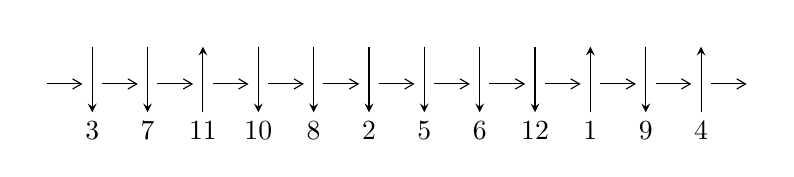
\begin{tikzpicture}[x=20pt, y=17pt]
	% nodes
	\node (C0) at (0, 0) {};
	\node (C1) at (1, 0) {};
	\node (C1U) at (1, +1) {};
	\node (C1D) at (1, -1) {3};

	\node (C2) at (2, 0) {};
	\node (C2U) at (2, +1) {};
	\node (C2D) at (2, -1) {7};

	\node (C3) at (3, 0) {};
	\node (C3U) at (3, +1) {};
	\node (C3D) at (3, -1) {11};

	\node (C4) at (4, 0) {};
	\node (C4U) at (4, +1) {};
	\node (C4D) at (4, -1) {10};

	\node (C5) at (5, 0) {};
	\node (C5U) at (5, +1) {};
	\node (C5D) at (5, -1) {8};

	\node (C6) at (6, 0) {};
	\node (C6U) at (6, +1) {};
	\node (C6D) at (6, -1) {2};

	\node (C7) at (7, 0) {};
	\node (C7U) at (7, +1) {};
	\node (C7D) at (7, -1) {5};

	\node (C8) at (8, 0) {};
	\node (C8U) at (8, +1) {};
	\node (C8D) at (8, -1) {6};

	\node (C9) at (9, 0) {};
	\node (C9U) at (9, +1) {};
	\node (C9D) at (9, -1) {12};

	\node (C10) at (10, 0) {};
	\node (C10U) at (10, +1) {};
	\node (C10D) at (10, -1) {1};

	\node (C11) at (11, 0) {};
	\node (C11U) at (11, +1) {};
	\node (C11D) at (11, -1) {9};

	\node (C12) at (12, 0) {};
	\node (C12U) at (12, +1) {};
	\node (C12D) at (12, -1) {4};
	\node (C13) at (13, 0) {};

	% arrows
	\draw[->,>={angle 60}]
	(C0) edge (C1) (C1) edge (C2) (C2) edge (C3) (C3) edge (C4) (C4) edge (C5) (C5) edge (C6) (C6) edge (C7) (C7) edge (C8) (C8) edge (C9) (C9) edge (C10) (C10) edge (C11) (C11) edge (C12) (C12) edge (C13) ;	\draw[->,>=stealth]
	(C1U) edge (C1D) (C2U) edge (C2D) (C3D) edge (C3U) (C4U) edge (C4D) (C5U) edge (C5D) (C6U) edge (C6D) (C7U) edge (C7D) (C8U) edge (C8D) (C9U) edge (C9D) (C10D) edge (C10U) (C11U) edge (C11D) (C12D) edge (C12U) ;
	\end{tikzpicture} \\
\hhline{~~} \\& 
\textbf{Solving Sequence} \\ \cline{2-2} 
 &
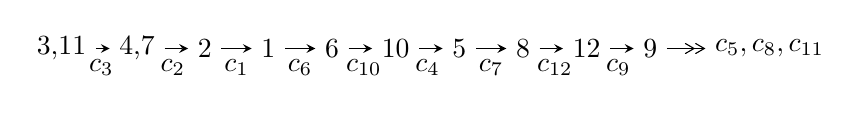
\begin{tikzpicture}[x=23pt, y=7pt]
	% node
	\node (A0) at (-1/8, 0) {3,11};
	\node (A1) at (17/16, 0) {4,7};
	\node (A2) at (17/8, 0) {2};
	\node (A3) at (25/8, 0) {1};
	\node (A4) at (33/8, 0) {6};
	\node (A5) at (41/8, 0) {10};
	\node (A6) at (49/8, 0) {5};
	\node (A7) at (57/8, 0) {8};
	\node (A8) at (65/8, 0) {12};
	\node (A9) at (73/8, 0) {9};
	\node (C1) at (1/2, -1) {$c_{3}$};
	\node (C2) at (13/8, -1) {$c_{2}$};
	\node (C3) at (21/8, -1) {$c_{1}$};
	\node (C4) at (29/8, -1) {$c_{6}$};
	\node (C5) at (37/8, -1) {$c_{10}$};
	\node (C6) at (45/8, -1) {$c_{4}$};
	\node (C7) at (53/8, -1) {$c_{7}$};
	\node (C8) at (61/8, -1) {$c_{12}$};
	\node (C9) at (69/8, -1) {$c_{9}$};
	\node (A10) at (11, 0) {$c_{5},c_{8},c_{11}$};

	% edge
	\draw[->,>=stealth]	
	(A0) edge (A1) (A1) edge (A2) (A2) edge (A3) (A3) edge (A4) (A4) edge (A5) (A5) edge (A6) (A6) edge (A7) (A7) edge (A8) (A8) edge (A9) ;
	\draw[->>,>={angle 60}]	
	(A9) edge (A10);
\end{tikzpicture} \\ 

\end{tabular} \\

\footnotetext{
The image of knot diagram is generated by the software ``\textbf{Draw programme}" developed by Andrew Bartholomew(\url{http://www.layer8.co.uk/maths/draw/index.htm\#Running-draw}), where we modified some parts for our purpose(\url{https://github.com/CATsTAILs/LinksPainter}).
}\phantom \\ \newline 
\centering \textbf{Ideals for irreducible components\footnotemark of $X_{\text{par}}$} 
 
\begin{align*}
I^u_{1}&=\langle 
8.64413\times10^{873} u^{111}-4.69059\times10^{874} u^{110}+\cdots+2.10211\times10^{875} b+3.17682\times10^{876},\\
\phantom{I^u_{1}}&\phantom{= \langle  }2.94142\times10^{875} u^{111}-1.73846\times10^{876} u^{110}+\cdots+3.38440\times10^{877} a+5.18415\times10^{878},\\
\phantom{I^u_{1}}&\phantom{= \langle  }u^{112}-5 u^{111}+\cdots-32 u+161\rangle \\
I^u_{2}&=\langle 
b,\;u^5+2 u^4- u^3-3 u^2+a+2,\;u^6+u^5- u^4-2 u^3+u+1\rangle \\
I^u_{3}&=\langle 
b+u+2,\;a-1,\;u^2+3 u+1\rangle \\
\\
\end{align*}
\raggedright * 3 irreducible components of $\dim_{\mathbb{C}}=0$, with total 120 representations.\\
\footnotetext{All coefficients of polynomials are rational numbers. But the coefficients are sometimes approximated in decimal forms when there is not enough margin.}
\newpage
\renewcommand{\arraystretch}{1}
\centering \section*{I. $I^u_{1}= \langle 8.64\times10^{873} u^{111}-4.69\times10^{874} u^{110}+\cdots+2.10\times10^{875} b+3.18\times10^{876},\;2.94\times10^{875} u^{111}-1.74\times10^{876} u^{110}+\cdots+3.38\times10^{877} a+5.18\times10^{878},\;u^{112}-5 u^{111}+\cdots-32 u+161 \rangle$}
\flushleft \textbf{(i) Arc colorings}\\
\begin{tabular}{m{7pt} m{180pt} m{7pt} m{180pt} }
\flushright $a_{3}=$&$\begin{pmatrix}1\\0\end{pmatrix}$ \\
\flushright $a_{11}=$&$\begin{pmatrix}0\\u\end{pmatrix}$ \\
\flushright $a_{4}=$&$\begin{pmatrix}1\\- u^2\end{pmatrix}$ \\
\flushright $a_{7}=$&$\begin{pmatrix}-0.00869112 u^{111}+0.0513670 u^{110}+\cdots-22.1084 u-15.3178\\-0.0411212 u^{111}+0.223137 u^{110}+\cdots+49.0131 u-15.1125\end{pmatrix}$ \\
\flushright $a_{2}=$&$\begin{pmatrix}0.0417015 u^{111}-0.223931 u^{110}+\cdots-1.70906 u+19.4928\\-0.0475784 u^{111}+0.258130 u^{110}+\cdots+41.4609 u-18.2032\end{pmatrix}$ \\
\flushright $a_{1}=$&$\begin{pmatrix}-0.00587685 u^{111}+0.0341992 u^{110}+\cdots+39.7519 u+1.28959\\-0.0475784 u^{111}+0.258130 u^{110}+\cdots+41.4609 u-18.2032\end{pmatrix}$ \\
\flushright $a_{6}=$&$\begin{pmatrix}-0.0777167 u^{111}+0.428161 u^{110}+\cdots+64.6212 u-43.6433\\0.0560739 u^{111}-0.303666 u^{110}+\cdots-49.2634 u+20.8838\end{pmatrix}$ \\
\flushright $a_{10}=$&$\begin{pmatrix}-0.0139652 u^{111}+0.0715977 u^{110}+\cdots+10.2906 u+6.50129\\0.0156815 u^{111}-0.0832120 u^{110}+\cdots-16.6168 u+3.89101\end{pmatrix}$ \\
\flushright $a_{5}=$&$\begin{pmatrix}0.00952388 u^{111}-0.0439959 u^{110}+\cdots+1.32330 u-3.32008\\0.000290774 u^{111}-0.00392329 u^{110}+\cdots+0.729889 u+1.77651\end{pmatrix}$ \\
\flushright $a_{8}=$&$\begin{pmatrix}0.0324993 u^{111}-0.172787 u^{110}+\cdots-30.0523 u+8.35382\\-0.0466259 u^{111}+0.252618 u^{110}+\cdots+49.2139 u-17.8341\end{pmatrix}$ \\
\flushright $a_{12}=$&$\begin{pmatrix}0.0424410 u^{111}-0.227744 u^{110}+\cdots-2.80931 u+20.2680\\-0.0567134 u^{111}+0.307789 u^{110}+\cdots+49.8914 u-21.4801\end{pmatrix}$ \\
\flushright $a_{9}=$&$\begin{pmatrix}0.0353301 u^{111}-0.195586 u^{110}+\cdots-74.1382 u+16.7074\\-0.0486125 u^{111}+0.264384 u^{110}+\cdots+48.8205 u-20.2064\end{pmatrix}$\\&\end{tabular}
\flushleft \textbf{(ii) Obstruction class $= -1$}\\~\\
\flushleft \textbf{(iii) Cusp Shapes $= 1.30472 u^{111}-7.06537 u^{110}+\cdots-1339.89 u+498.199$}\\~\\
\newpage\renewcommand{\arraystretch}{1}
\flushleft \textbf{(iv) u-Polynomials at the component}\newline \\
\begin{tabular}{m{50pt}|m{274pt}}
Crossings & \hspace{64pt}u-Polynomials at each crossing \\
\hline $$\begin{aligned}c_{1}\end{aligned}$$&$\begin{aligned}
&u^{112}+42 u^{111}+\cdots+36864 u+4096
\end{aligned}$\\
\hline $$\begin{aligned}c_{2},c_{6}\end{aligned}$$&$\begin{aligned}
&u^{112}-2 u^{111}+\cdots+192 u+64
\end{aligned}$\\
\hline $$\begin{aligned}c_{3}\end{aligned}$$&$\begin{aligned}
&u^{112}-5 u^{111}+\cdots-32 u+161
\end{aligned}$\\
\hline $$\begin{aligned}c_{4}\end{aligned}$$&$\begin{aligned}
&u^{112}-9 u^{111}+\cdots+2324 u-121
\end{aligned}$\\
\hline $$\begin{aligned}c_{5},c_{7},c_{8}\end{aligned}$$&$\begin{aligned}
&u^{112}-8 u^{111}+\cdots-7 u+1
\end{aligned}$\\
\hline $$\begin{aligned}c_{9},c_{11}\end{aligned}$$&$\begin{aligned}
&u^{112}-4 u^{111}+\cdots-35 u+1
\end{aligned}$\\
\hline $$\begin{aligned}c_{10}\end{aligned}$$&$\begin{aligned}
&u^{112}+18 u^{111}+\cdots-48 u+4
\end{aligned}$\\
\hline $$\begin{aligned}c_{12}\end{aligned}$$&$\begin{aligned}
&u^{112}+9 u^{111}+\cdots+2 u+1
\end{aligned}$\\
\hline
\end{tabular}\\~\\
\newpage\renewcommand{\arraystretch}{1}
\flushleft \textbf{(v) Riley Polynomials at the component}\newline \\
\begin{tabular}{m{50pt}|m{274pt}}
Crossings & \hspace{64pt}Riley Polynomials at each crossing \\
\hline $$\begin{aligned}c_{1}\end{aligned}$$&$\begin{aligned}
&y^{112}+46 y^{111}+\cdots+1719664640 y+16777216
\end{aligned}$\\
\hline $$\begin{aligned}c_{2},c_{6}\end{aligned}$$&$\begin{aligned}
&y^{112}-42 y^{111}+\cdots-36864 y+4096
\end{aligned}$\\
\hline $$\begin{aligned}c_{3}\end{aligned}$$&$\begin{aligned}
&y^{112}-109 y^{111}+\cdots-254760 y+25921
\end{aligned}$\\
\hline $$\begin{aligned}c_{4}\end{aligned}$$&$\begin{aligned}
&y^{112}-109 y^{111}+\cdots-1162588 y+14641
\end{aligned}$\\
\hline $$\begin{aligned}c_{5},c_{7},c_{8}\end{aligned}$$&$\begin{aligned}
&y^{112}-96 y^{111}+\cdots+115 y+1
\end{aligned}$\\
\hline $$\begin{aligned}c_{9},c_{11}\end{aligned}$$&$\begin{aligned}
&y^{112}-68 y^{111}+\cdots-815 y+1
\end{aligned}$\\
\hline $$\begin{aligned}c_{10}\end{aligned}$$&$\begin{aligned}
&y^{112}-18 y^{111}+\cdots-1464 y+16
\end{aligned}$\\
\hline $$\begin{aligned}c_{12}\end{aligned}$$&$\begin{aligned}
&y^{112}+11 y^{111}+\cdots-8 y+1
\end{aligned}$\\
\hline
\end{tabular}\\~\\
\newpage\flushleft \textbf{(vi) Complex Volumes and Cusp Shapes}
$$\begin{array}{c|c|c}  
\text{Solutions to }I^u_{1}& \I (\text{vol} + \sqrt{-1}CS) & \text{Cusp shape}\\
 \hline 
\begin{aligned}
u &= -0.468045 + 0.892905 I \\
a &= -0.13957 - 1.52043 I \\
b &= \phantom{-}1.212340 + 0.047993 I\end{aligned}
 & -10.99840 - 2.00997 I & \phantom{-0.000000 } 0 \\ \hline\begin{aligned}
u &= -0.468045 - 0.892905 I \\
a &= -0.13957 + 1.52043 I \\
b &= \phantom{-}1.212340 - 0.047993 I\end{aligned}
 & -10.99840 + 2.00997 I & \phantom{-0.000000 } 0 \\ \hline\begin{aligned}
u &= \phantom{-}1.026540 + 0.095270 I \\
a &= \phantom{-}0.531056 + 0.969905 I \\
b &= -0.541459 - 0.797677 I\end{aligned}
 & \phantom{-}3.07753 + 0.68921 I & \phantom{-0.000000 } 0 \\ \hline\begin{aligned}
u &= \phantom{-}1.026540 - 0.095270 I \\
a &= \phantom{-}0.531056 - 0.969905 I \\
b &= -0.541459 + 0.797677 I\end{aligned}
 & \phantom{-}3.07753 - 0.68921 I & \phantom{-0.000000 } 0 \\ \hline\begin{aligned}
u &= \phantom{-}0.474652 + 0.832338 I \\
a &= \phantom{-}0.501877 - 0.671501 I \\
b &= \phantom{-}1.149220 + 0.205342 I\end{aligned}
 & -4.72741 + 2.38013 I & \phantom{-0.000000 } 0 \\ \hline\begin{aligned}
u &= \phantom{-}0.474652 - 0.832338 I \\
a &= \phantom{-}0.501877 + 0.671501 I \\
b &= \phantom{-}1.149220 - 0.205342 I\end{aligned}
 & -4.72741 - 2.38013 I & \phantom{-0.000000 } 0 \\ \hline\begin{aligned}
u &= -0.986400 + 0.352157 I \\
a &= -0.06333 + 1.49320 I \\
b &= -1.095380 - 0.664874 I\end{aligned}
 & \phantom{-}1.39228 - 6.23151 I & \phantom{-0.000000 } 0 \\ \hline\begin{aligned}
u &= -0.986400 - 0.352157 I \\
a &= -0.06333 - 1.49320 I \\
b &= -1.095380 + 0.664874 I\end{aligned}
 & \phantom{-}1.39228 + 6.23151 I & \phantom{-0.000000 } 0 \\ \hline\begin{aligned}
u &= -0.439969 + 0.844782 I \\
a &= \phantom{-}0.750760 + 0.662615 I \\
b &= \phantom{-}0.168122 - 0.261520 I\end{aligned}
 & -1.92777 + 0.81004 I & \phantom{-0.000000 } 0 \\ \hline\begin{aligned}
u &= -0.439969 - 0.844782 I \\
a &= \phantom{-}0.750760 - 0.662615 I \\
b &= \phantom{-}0.168122 + 0.261520 I\end{aligned}
 & -1.92777 - 0.81004 I & \phantom{-0.000000 } 0\\
 \hline 
 \end{array}$$\newpage$$\begin{array}{c|c|c}  
\text{Solutions to }I^u_{1}& \I (\text{vol} + \sqrt{-1}CS) & \text{Cusp shape}\\
 \hline 
\begin{aligned}
u &= \phantom{-}0.900349 + 0.307525 I \\
a &= -0.58166 - 1.29875 I \\
b &= \phantom{-}0.564295 + 1.113070 I\end{aligned}
 & -1.81857 + 4.04926 I & \phantom{-0.000000 } 0 \\ \hline\begin{aligned}
u &= \phantom{-}0.900349 - 0.307525 I \\
a &= -0.58166 + 1.29875 I \\
b &= \phantom{-}0.564295 - 1.113070 I\end{aligned}
 & -1.81857 - 4.04926 I & \phantom{-0.000000 } 0 \\ \hline\begin{aligned}
u &= \phantom{-}0.305901 + 0.888362 I \\
a &= \phantom{-}0.236205 + 1.086070 I \\
b &= \phantom{-}1.045770 - 0.734544 I\end{aligned}
 & -1.43150 + 7.30797 I & \phantom{-0.000000 } 0 \\ \hline\begin{aligned}
u &= \phantom{-}0.305901 - 0.888362 I \\
a &= \phantom{-}0.236205 - 1.086070 I \\
b &= \phantom{-}1.045770 + 0.734544 I\end{aligned}
 & -1.43150 - 7.30797 I & \phantom{-0.000000 } 0 \\ \hline\begin{aligned}
u &= \phantom{-}0.866434 + 0.319209 I \\
a &= \phantom{-}0.281117 + 0.511404 I \\
b &= -0.085748 - 0.495139 I\end{aligned}
 & \phantom{-}1.46476 + 1.15131 I & \phantom{-0.000000 } 0 \\ \hline\begin{aligned}
u &= \phantom{-}0.866434 - 0.319209 I \\
a &= \phantom{-}0.281117 - 0.511404 I \\
b &= -0.085748 + 0.495139 I\end{aligned}
 & \phantom{-}1.46476 - 1.15131 I & \phantom{-0.000000 } 0 \\ \hline\begin{aligned}
u &= \phantom{-}0.113281 + 1.084940 I \\
a &= -1.16785 - 1.00702 I \\
b &= -0.351973 + 0.831284 I\end{aligned}
 & -5.29466 - 0.57195 I & \phantom{-0.000000 } 0 \\ \hline\begin{aligned}
u &= \phantom{-}0.113281 - 1.084940 I \\
a &= -1.16785 + 1.00702 I \\
b &= -0.351973 - 0.831284 I\end{aligned}
 & -5.29466 + 0.57195 I & \phantom{-0.000000 } 0 \\ \hline\begin{aligned}
u &= -0.088142 + 0.899059 I \\
a &= -1.61631 + 1.18838 I \\
b &= -0.757971 + 0.094539 I\end{aligned}
 & -4.28499 - 1.36074 I & \phantom{-0.000000 } 0 \\ \hline\begin{aligned}
u &= -0.088142 - 0.899059 I \\
a &= -1.61631 - 1.18838 I \\
b &= -0.757971 - 0.094539 I\end{aligned}
 & -4.28499 + 1.36074 I & \phantom{-0.000000 } 0\\
 \hline 
 \end{array}$$\newpage$$\begin{array}{c|c|c}  
\text{Solutions to }I^u_{1}& \I (\text{vol} + \sqrt{-1}CS) & \text{Cusp shape}\\
 \hline 
\begin{aligned}
u &= -0.566275 + 0.948690 I \\
a &= \phantom{-}0.209851 + 1.205160 I \\
b &= -0.070911 - 1.168160 I\end{aligned}
 & -6.89574 - 4.83025 I & \phantom{-0.000000 } 0 \\ \hline\begin{aligned}
u &= -0.566275 - 0.948690 I \\
a &= \phantom{-}0.209851 - 1.205160 I \\
b &= -0.070911 + 1.168160 I\end{aligned}
 & -6.89574 + 4.83025 I & \phantom{-0.000000 } 0 \\ \hline\begin{aligned}
u &= \phantom{-}0.105634 + 0.883669 I \\
a &= \phantom{-}0.142577 + 0.894261 I \\
b &= -1.38242 - 0.36899 I\end{aligned}
 & -11.58490 - 0.78846 I & \phantom{-0.000000 } 0 \\ \hline\begin{aligned}
u &= \phantom{-}0.105634 - 0.883669 I \\
a &= \phantom{-}0.142577 - 0.894261 I \\
b &= -1.38242 + 0.36899 I\end{aligned}
 & -11.58490 + 0.78846 I & \phantom{-0.000000 } 0 \\ \hline\begin{aligned}
u &= -0.861494 + 0.198796 I \\
a &= \phantom{-}0.369814 - 1.123050 I \\
b &= \phantom{-}1.052340 + 0.440204 I\end{aligned}
 & -0.97322 - 1.18405 I & \phantom{-0.000000 } 0 \\ \hline\begin{aligned}
u &= -0.861494 - 0.198796 I \\
a &= \phantom{-}0.369814 + 1.123050 I \\
b &= \phantom{-}1.052340 - 0.440204 I\end{aligned}
 & -0.97322 + 1.18405 I & \phantom{-0.000000 } 0 \\ \hline\begin{aligned}
u &= -0.911716 + 0.662167 I \\
a &= -0.114233 - 0.615496 I \\
b &= \phantom{-}0.029697 + 0.635113 I\end{aligned}
 & -0.90850 - 5.42294 I & \phantom{-0.000000 } 0 \\ \hline\begin{aligned}
u &= -0.911716 - 0.662167 I \\
a &= -0.114233 + 0.615496 I \\
b &= \phantom{-}0.029697 - 0.635113 I\end{aligned}
 & -0.90850 + 5.42294 I & \phantom{-0.000000 } 0 \\ \hline\begin{aligned}
u &= -0.390502 + 0.770194 I \\
a &= \phantom{-}1.182600 - 0.418464 I \\
b &= \phantom{-}1.178770 + 0.169202 I\end{aligned}
 & -7.09262 - 4.86963 I & \phantom{-0.000000 } 0 \\ \hline\begin{aligned}
u &= -0.390502 - 0.770194 I \\
a &= \phantom{-}1.182600 + 0.418464 I \\
b &= \phantom{-}1.178770 - 0.169202 I\end{aligned}
 & -7.09262 + 4.86963 I & \phantom{-0.000000 } 0\\
 \hline 
 \end{array}$$\newpage$$\begin{array}{c|c|c}  
\text{Solutions to }I^u_{1}& \I (\text{vol} + \sqrt{-1}CS) & \text{Cusp shape}\\
 \hline 
\begin{aligned}
u &= -0.855537 + 0.095153 I \\
a &= -0.736687 + 0.424172 I \\
b &= \phantom{-}0.824062 - 0.686417 I\end{aligned}
 & -0.18525 + 6.98643 I & \phantom{-0.000000 } 0 \\ \hline\begin{aligned}
u &= -0.855537 - 0.095153 I \\
a &= -0.736687 - 0.424172 I \\
b &= \phantom{-}0.824062 + 0.686417 I\end{aligned}
 & -0.18525 - 6.98643 I & \phantom{-0.000000 } 0 \\ \hline\begin{aligned}
u &= -1.036730 + 0.484104 I \\
a &= -0.15871 - 1.57266 I \\
b &= \phantom{-}1.180290 + 0.770211 I\end{aligned}
 & -3.79919 - 10.78570 I & \phantom{-0.000000 } 0 \\ \hline\begin{aligned}
u &= -1.036730 - 0.484104 I \\
a &= -0.15871 + 1.57266 I \\
b &= \phantom{-}1.180290 - 0.770211 I\end{aligned}
 & -3.79919 + 10.78570 I & \phantom{-0.000000 } 0 \\ \hline\begin{aligned}
u &= -0.878136 + 0.769471 I \\
a &= -1.03073 + 1.75744 I \\
b &= -0.854510 - 0.585436 I\end{aligned}
 & \phantom{-}0.97833 - 3.36110 I & \phantom{-0.000000 } 0 \\ \hline\begin{aligned}
u &= -0.878136 - 0.769471 I \\
a &= -1.03073 - 1.75744 I \\
b &= -0.854510 + 0.585436 I\end{aligned}
 & \phantom{-}0.97833 + 3.36110 I & \phantom{-0.000000 } 0 \\ \hline\begin{aligned}
u &= -0.705292 + 0.964759 I \\
a &= -0.134401 + 0.171016 I \\
b &= -1.104990 + 0.102541 I\end{aligned}
 & -6.88250 + 0.95679 I & \phantom{-0.000000 } 0 \\ \hline\begin{aligned}
u &= -0.705292 - 0.964759 I \\
a &= -0.134401 - 0.171016 I \\
b &= -1.104990 - 0.102541 I\end{aligned}
 & -6.88250 - 0.95679 I & \phantom{-0.000000 } 0 \\ \hline\begin{aligned}
u &= -0.102997 + 1.191740 I \\
a &= \phantom{-}0.718781 + 0.113606 I \\
b &= \phantom{-}0.872881 - 0.545073 I\end{aligned}
 & -2.51350 + 2.16509 I & \phantom{-0.000000 } 0 \\ \hline\begin{aligned}
u &= -0.102997 - 1.191740 I \\
a &= \phantom{-}0.718781 - 0.113606 I \\
b &= \phantom{-}0.872881 + 0.545073 I\end{aligned}
 & -2.51350 - 2.16509 I & \phantom{-0.000000 } 0\\
 \hline 
 \end{array}$$\newpage$$\begin{array}{c|c|c}  
\text{Solutions to }I^u_{1}& \I (\text{vol} + \sqrt{-1}CS) & \text{Cusp shape}\\
 \hline 
\begin{aligned}
u &= \phantom{-}0.853382 + 0.851081 I \\
a &= \phantom{-}0.666579 + 0.635943 I \\
b &= -0.618439 - 0.951660 I\end{aligned}
 & \phantom{-}0.51258 + 6.03565 I & \phantom{-0.000000 } 0 \\ \hline\begin{aligned}
u &= \phantom{-}0.853382 - 0.851081 I \\
a &= \phantom{-}0.666579 - 0.635943 I \\
b &= -0.618439 + 0.951660 I\end{aligned}
 & \phantom{-}0.51258 - 6.03565 I & \phantom{-0.000000 } 0 \\ \hline\begin{aligned}
u &= \phantom{-}0.698002 + 0.997090 I \\
a &= -0.616237 - 0.033041 I \\
b &= -1.124740 + 0.060024 I\end{aligned}
 & -5.03852 + 7.34388 I & \phantom{-0.000000 } 0 \\ \hline\begin{aligned}
u &= \phantom{-}0.698002 - 0.997090 I \\
a &= -0.616237 + 0.033041 I \\
b &= -1.124740 - 0.060024 I\end{aligned}
 & -5.03852 - 7.34388 I & \phantom{-0.000000 } 0 \\ \hline\begin{aligned}
u &= -0.584208 + 0.484004 I \\
a &= -1.85886 + 0.99076 I \\
b &= -0.852044 - 0.127697 I\end{aligned}
 & -0.94679 - 3.25376 I & \phantom{-0.000000 } 0 \\ \hline\begin{aligned}
u &= -0.584208 - 0.484004 I \\
a &= -1.85886 - 0.99076 I \\
b &= -0.852044 + 0.127697 I\end{aligned}
 & -0.94679 + 3.25376 I & \phantom{-0.000000 } 0 \\ \hline\begin{aligned}
u &= \phantom{-}0.993124 + 0.771280 I \\
a &= -0.761129 - 0.522135 I \\
b &= \phantom{-}0.705432 + 0.773381 I\end{aligned}
 & \phantom{-}4.67418 + 2.34341 I & \phantom{-0.000000 } 0 \\ \hline\begin{aligned}
u &= \phantom{-}0.993124 - 0.771280 I \\
a &= -0.761129 + 0.522135 I \\
b &= \phantom{-}0.705432 - 0.773381 I\end{aligned}
 & \phantom{-}4.67418 - 2.34341 I & \phantom{-0.000000 } 0 \\ \hline\begin{aligned}
u &= \phantom{-}1.255610 + 0.094001 I \\
a &= -0.781393 + 0.562496 I \\
b &= \phantom{-}0.784331 - 0.418208 I\end{aligned}
 & -0.04609 + 2.27832 I & \phantom{-0.000000 } 0 \\ \hline\begin{aligned}
u &= \phantom{-}1.255610 - 0.094001 I \\
a &= -0.781393 - 0.562496 I \\
b &= \phantom{-}0.784331 + 0.418208 I\end{aligned}
 & -0.04609 - 2.27832 I & \phantom{-0.000000 } 0\\
 \hline 
 \end{array}$$\newpage$$\begin{array}{c|c|c}  
\text{Solutions to }I^u_{1}& \I (\text{vol} + \sqrt{-1}CS) & \text{Cusp shape}\\
 \hline 
\begin{aligned}
u &= -0.891203 + 0.911299 I \\
a &= \phantom{-}0.67375 - 1.67146 I \\
b &= \phantom{-}0.985762 + 0.695082 I\end{aligned}
 & \phantom{-}3.81295 - 7.90390 I & \phantom{-0.000000 } 0 \\ \hline\begin{aligned}
u &= -0.891203 - 0.911299 I \\
a &= \phantom{-}0.67375 + 1.67146 I \\
b &= \phantom{-}0.985762 - 0.695082 I\end{aligned}
 & \phantom{-}3.81295 + 7.90390 I & \phantom{-0.000000 } 0 \\ \hline\begin{aligned}
u &= \phantom{-}0.278553 + 0.649349 I \\
a &= -0.543784 - 1.113530 I \\
b &= -0.927060 + 0.744372 I\end{aligned}
 & \phantom{-}3.10964 + 3.02719 I & \phantom{-0.000000 } 0 \\ \hline\begin{aligned}
u &= \phantom{-}0.278553 - 0.649349 I \\
a &= -0.543784 + 1.113530 I \\
b &= -0.927060 - 0.744372 I\end{aligned}
 & \phantom{-}3.10964 - 3.02719 I & \phantom{-0.000000 } 0 \\ \hline\begin{aligned}
u &= -0.197409 + 1.284420 I \\
a &= -0.223939 - 0.085915 I \\
b &= -1.094380 + 0.606228 I\end{aligned}
 & -7.43290 + 5.78346 I & \phantom{-0.000000 } 0 \\ \hline\begin{aligned}
u &= -0.197409 - 1.284420 I \\
a &= -0.223939 + 0.085915 I \\
b &= -1.094380 - 0.606228 I\end{aligned}
 & -7.43290 - 5.78346 I & \phantom{-0.000000 } 0 \\ \hline\begin{aligned}
u &= -0.590165 + 0.343631 I \\
a &= \phantom{-}1.47450 + 2.91661 I \\
b &= -1.107300 - 0.670157 I\end{aligned}
 & -6.26355 - 9.78611 I & \phantom{-0.000000 } 0 \\ \hline\begin{aligned}
u &= -0.590165 - 0.343631 I \\
a &= \phantom{-}1.47450 - 2.91661 I \\
b &= -1.107300 + 0.670157 I\end{aligned}
 & -6.26355 + 9.78611 I & \phantom{-0.000000 } 0 \\ \hline\begin{aligned}
u &= -0.869024 + 1.011960 I \\
a &= -0.47159 + 1.56244 I \\
b &= -1.098070 - 0.735726 I\end{aligned}
 & -1.00529 - 12.22180 I & \phantom{-0.000000 } 0 \\ \hline\begin{aligned}
u &= -0.869024 - 1.011960 I \\
a &= -0.47159 - 1.56244 I \\
b &= -1.098070 + 0.735726 I\end{aligned}
 & -1.00529 + 12.22180 I & \phantom{-0.000000 } 0\\
 \hline 
 \end{array}$$\newpage$$\begin{array}{c|c|c}  
\text{Solutions to }I^u_{1}& \I (\text{vol} + \sqrt{-1}CS) & \text{Cusp shape}\\
 \hline 
\begin{aligned}
u &= -0.588740 + 0.308270 I \\
a &= \phantom{-}1.42258 - 0.40347 I \\
b &= \phantom{-}0.730002 - 0.053014 I\end{aligned}
 & -1.135370 + 0.042892 I & \phantom{-0.000000 } 0 \\ \hline\begin{aligned}
u &= -0.588740 - 0.308270 I \\
a &= \phantom{-}1.42258 + 0.40347 I \\
b &= \phantom{-}0.730002 + 0.053014 I\end{aligned}
 & -1.135370 - 0.042892 I & \phantom{-0.000000 } 0 \\ \hline\begin{aligned}
u &= \phantom{-}0.560265 + 0.316560 I \\
a &= -1.042770 - 0.669832 I \\
b &= \phantom{-}0.004601 + 0.787819 I\end{aligned}
 & -2.72849 + 1.53038 I & \phantom{-0.000000 } 0 \\ \hline\begin{aligned}
u &= \phantom{-}0.560265 - 0.316560 I \\
a &= -1.042770 + 0.669832 I \\
b &= \phantom{-}0.004601 - 0.787819 I\end{aligned}
 & -2.72849 - 1.53038 I & \phantom{-0.000000 } 0 \\ \hline\begin{aligned}
u &= \phantom{-}1.165230 + 0.702845 I \\
a &= \phantom{-}0.891880 + 0.374546 I \\
b &= -0.857228 - 0.576973 I\end{aligned}
 & \phantom{-}0.97470 - 1.25354 I & \phantom{-0.000000 } 0 \\ \hline\begin{aligned}
u &= \phantom{-}1.165230 - 0.702845 I \\
a &= \phantom{-}0.891880 - 0.374546 I \\
b &= -0.857228 + 0.576973 I\end{aligned}
 & \phantom{-}0.97470 + 1.25354 I & \phantom{-0.000000 } 0 \\ \hline\begin{aligned}
u &= -0.110576 + 0.543663 I \\
a &= \phantom{-}0.300944 + 0.690223 I \\
b &= \phantom{-}0.712854 - 0.837133 I\end{aligned}
 & -0.359065 - 1.357260 I & -4.82662 + 0. I\phantom{ +0.000000I} \\ \hline\begin{aligned}
u &= -0.110576 - 0.543663 I \\
a &= \phantom{-}0.300944 - 0.690223 I \\
b &= \phantom{-}0.712854 + 0.837133 I\end{aligned}
 & -0.359065 + 1.357260 I & -4.82662 + 0. I\phantom{ +0.000000I} \\ \hline\begin{aligned}
u &= \phantom{-}0.349469 + 0.426717 I \\
a &= \phantom{-}2.77883 + 2.17565 I \\
b &= -0.497376 - 0.903947 I\end{aligned}
 & -4.39307 + 4.01879 I & -13.0394 - 6.3418 I \\ \hline\begin{aligned}
u &= \phantom{-}0.349469 - 0.426717 I \\
a &= \phantom{-}2.77883 - 2.17565 I \\
b &= -0.497376 + 0.903947 I\end{aligned}
 & -4.39307 - 4.01879 I & -13.0394 + 6.3418 I\\
 \hline 
 \end{array}$$\newpage$$\begin{array}{c|c|c}  
\text{Solutions to }I^u_{1}& \I (\text{vol} + \sqrt{-1}CS) & \text{Cusp shape}\\
 \hline 
\begin{aligned}
u &= -0.492698 + 0.239422 I \\
a &= \phantom{-}0.549744 - 0.276436 I \\
b &= -0.800248 + 0.836455 I\end{aligned}
 & \phantom{-}3.50998 + 2.86593 I & -0.44864 - 5.27046 I \\ \hline\begin{aligned}
u &= -0.492698 - 0.239422 I \\
a &= \phantom{-}0.549744 + 0.276436 I \\
b &= -0.800248 - 0.836455 I\end{aligned}
 & \phantom{-}3.50998 - 2.86593 I & -0.44864 + 5.27046 I \\ \hline\begin{aligned}
u &= -0.429062 + 0.334358 I \\
a &= -1.24655 - 3.63053 I \\
b &= \phantom{-}0.948423 + 0.616190 I\end{aligned}
 & -1.33438 - 5.79082 I & -9.77157 + 8.99738 I \\ \hline\begin{aligned}
u &= -0.429062 - 0.334358 I \\
a &= -1.24655 + 3.63053 I \\
b &= \phantom{-}0.948423 - 0.616190 I\end{aligned}
 & -1.33438 + 5.79082 I & -9.77157 - 8.99738 I \\ \hline\begin{aligned}
u &= -0.160167 + 0.470619 I \\
a &= -0.97937 + 4.21410 I \\
b &= -0.729051 - 0.393657 I\end{aligned}
 & -3.76699 - 1.68644 I & -14.6816 + 6.6415 I \\ \hline\begin{aligned}
u &= -0.160167 - 0.470619 I \\
a &= -0.97937 - 4.21410 I \\
b &= -0.729051 + 0.393657 I\end{aligned}
 & -3.76699 + 1.68644 I & -14.6816 - 6.6415 I \\ \hline\begin{aligned}
u &= \phantom{-}0.75840 + 1.30183 I \\
a &= \phantom{-}0.020758 + 0.437342 I \\
b &= \phantom{-}1.353180 - 0.264117 I\end{aligned}
 & -12.2107 + 9.8962 I & \phantom{-0.000000 } 0 \\ \hline\begin{aligned}
u &= \phantom{-}0.75840 - 1.30183 I \\
a &= \phantom{-}0.020758 - 0.437342 I \\
b &= \phantom{-}1.353180 + 0.264117 I\end{aligned}
 & -12.2107 - 9.8962 I & \phantom{-0.000000 } 0 \\ \hline\begin{aligned}
u &= -1.31955 + 0.74333 I \\
a &= \phantom{-}0.615027 - 0.525764 I \\
b &= -0.685413 + 0.484737 I\end{aligned}
 & -1.46335 - 4.79145 I & \phantom{-0.000000 } 0 \\ \hline\begin{aligned}
u &= -1.31955 - 0.74333 I \\
a &= \phantom{-}0.615027 + 0.525764 I \\
b &= -0.685413 - 0.484737 I\end{aligned}
 & -1.46335 + 4.79145 I & \phantom{-0.000000 } 0\\
 \hline 
 \end{array}$$\newpage$$\begin{array}{c|c|c}  
\text{Solutions to }I^u_{1}& \I (\text{vol} + \sqrt{-1}CS) & \text{Cusp shape}\\
 \hline 
\begin{aligned}
u &= -0.429439\phantom{ +0.000000I} \\
a &= \phantom{-}1.79353\phantom{ +0.000000I} \\
b &= \phantom{-}0.601087\phantom{ +0.000000I}\end{aligned}
 & -1.01489\phantom{ +0.000000I} & -10.1760\phantom{ +0.000000I} \\ \hline\begin{aligned}
u &= -1.22226 + 1.00947 I \\
a &= -0.531918 + 0.901402 I \\
b &= \phantom{-}0.616280 - 0.864859 I\end{aligned}
 & \phantom{-}1.47470 - 8.28591 I & \phantom{-0.000000 } 0 \\ \hline\begin{aligned}
u &= -1.22226 - 1.00947 I \\
a &= -0.531918 - 0.901402 I \\
b &= \phantom{-}0.616280 + 0.864859 I\end{aligned}
 & \phantom{-}1.47470 + 8.28591 I & \phantom{-0.000000 } 0 \\ \hline\begin{aligned}
u &= -0.414031\phantom{ +0.000000I} \\
a &= \phantom{-}0.710994\phantom{ +0.000000I} \\
b &= -1.65804\phantom{ +0.000000I}\end{aligned}
 & -10.4601\phantom{ +0.000000I} & \phantom{-}57.7740\phantom{ +0.000000I} \\ \hline\begin{aligned}
u &= \phantom{-}1.14674 + 1.11271 I \\
a &= -0.460592 - 1.320060 I \\
b &= -1.009770 + 0.565159 I\end{aligned}
 & -2.61261 + 9.14928 I & \phantom{-0.000000 } 0 \\ \hline\begin{aligned}
u &= \phantom{-}1.14674 - 1.11271 I \\
a &= -0.460592 + 1.320060 I \\
b &= -1.009770 - 0.565159 I\end{aligned}
 & -2.61261 - 9.14928 I & \phantom{-0.000000 } 0 \\ \hline\begin{aligned}
u &= -1.18789 + 1.17802 I \\
a &= \phantom{-}0.543314 - 1.107150 I \\
b &= -0.632118 + 1.066720 I\end{aligned}
 & -3.24903 - 12.04520 I & \phantom{-0.000000 } 0 \\ \hline\begin{aligned}
u &= -1.18789 - 1.17802 I \\
a &= \phantom{-}0.543314 + 1.107150 I \\
b &= -0.632118 - 1.066720 I\end{aligned}
 & -3.24903 + 12.04520 I & \phantom{-0.000000 } 0 \\ \hline\begin{aligned}
u &= \phantom{-}0.196988 + 0.216176 I \\
a &= -1.69062 - 5.29146 I \\
b &= -1.022500 + 0.540394 I\end{aligned}
 & -5.01539 + 2.29068 I & -12.66920 + 0.63312 I \\ \hline\begin{aligned}
u &= \phantom{-}0.196988 - 0.216176 I \\
a &= -1.69062 + 5.29146 I \\
b &= -1.022500 - 0.540394 I\end{aligned}
 & -5.01539 - 2.29068 I & -12.66920 - 0.63312 I\\
 \hline 
 \end{array}$$\newpage$$\begin{array}{c|c|c}  
\text{Solutions to }I^u_{1}& \I (\text{vol} + \sqrt{-1}CS) & \text{Cusp shape}\\
 \hline 
\begin{aligned}
u &= \phantom{-}0.201500 + 0.178702 I \\
a &= \phantom{-}1.82535 + 1.36786 I \\
b &= \phantom{-}0.857519 - 0.800677 I\end{aligned}
 & -0.28499 - 1.43055 I & -2.82816 + 2.44341 I \\ \hline\begin{aligned}
u &= \phantom{-}0.201500 - 0.178702 I \\
a &= \phantom{-}1.82535 - 1.36786 I \\
b &= \phantom{-}0.857519 + 0.800677 I\end{aligned}
 & -0.28499 + 1.43055 I & -2.82816 - 2.44341 I \\ \hline\begin{aligned}
u &= \phantom{-}1.25320 + 1.19672 I \\
a &= \phantom{-}0.19298 + 1.48373 I \\
b &= \phantom{-}1.067090 - 0.707773 I\end{aligned}
 & \phantom{-}0.0844 + 14.1422 I & \phantom{-0.000000 } 0 \\ \hline\begin{aligned}
u &= \phantom{-}1.25320 - 1.19672 I \\
a &= \phantom{-}0.19298 - 1.48373 I \\
b &= \phantom{-}1.067090 + 0.707773 I\end{aligned}
 & \phantom{-}0.0844 - 14.1422 I & \phantom{-0.000000 } 0 \\ \hline\begin{aligned}
u &= \phantom{-}0.137389 + 0.136164 I \\
a &= -7.22185 - 4.14942 I \\
b &= \phantom{-}0.702404 + 0.610926 I\end{aligned}
 & -0.591650 + 0.928319 I & -7.08998 - 2.83075 I \\ \hline\begin{aligned}
u &= \phantom{-}0.137389 - 0.136164 I \\
a &= -7.22185 + 4.14942 I \\
b &= \phantom{-}0.702404 - 0.610926 I\end{aligned}
 & -0.591650 - 0.928319 I & -7.08998 + 2.83075 I \\ \hline\begin{aligned}
u &= \phantom{-}1.30054 + 1.28561 I \\
a &= \phantom{-}0.00089 - 1.50453 I \\
b &= -1.148010 + 0.781264 I\end{aligned}
 & -4.9272 + 18.7232 I & \phantom{-0.000000 } 0 \\ \hline\begin{aligned}
u &= \phantom{-}1.30054 - 1.28561 I \\
a &= \phantom{-}0.00089 + 1.50453 I \\
b &= -1.148010 - 0.781264 I\end{aligned}
 & -4.9272 - 18.7232 I & \phantom{-0.000000 } 0 \\ \hline\begin{aligned}
u &= -2.08275 + 0.80093 I \\
a &= -0.267916 - 1.307150 I \\
b &= \phantom{-}1.018830 + 0.608303 I\end{aligned}
 & -3.83391 - 5.53172 I & \phantom{-0.000000 } 0 \\ \hline\begin{aligned}
u &= -2.08275 - 0.80093 I \\
a &= -0.267916 + 1.307150 I \\
b &= \phantom{-}1.018830 - 0.608303 I\end{aligned}
 & -3.83391 + 5.53172 I & \phantom{-0.000000 } 0\\
 \hline 
 \end{array}$$\newpage$$\begin{array}{c|c|c}  
\text{Solutions to }I^u_{1}& \I (\text{vol} + \sqrt{-1}CS) & \text{Cusp shape}\\
 \hline 
\begin{aligned}
u &= \phantom{-}2.25960 + 0.15223 I \\
a &= \phantom{-}0.04322 + 1.60132 I \\
b &= \phantom{-}0.572900 - 0.604567 I\end{aligned}
 & -2.52074 - 0.67374 I & \phantom{-0.000000 } 0 \\ \hline\begin{aligned}
u &= \phantom{-}2.25960 - 0.15223 I \\
a &= \phantom{-}0.04322 - 1.60132 I \\
b &= \phantom{-}0.572900 + 0.604567 I\end{aligned}
 & -2.52074 + 0.67374 I & \phantom{-0.000000 } 0 \\ \hline\begin{aligned}
u &= -2.26623 + 0.37498 I \\
a &= \phantom{-}0.08634 + 1.50403 I \\
b &= -0.800557 - 0.646744 I\end{aligned}
 & \phantom{-}0.63350 - 1.90492 I & \phantom{-0.000000 } 0 \\ \hline\begin{aligned}
u &= -2.26623 - 0.37498 I \\
a &= \phantom{-}0.08634 - 1.50403 I \\
b &= -0.800557 + 0.646744 I\end{aligned}
 & \phantom{-}0.63350 + 1.90492 I & \phantom{-0.000000 } 0 \\ \hline\begin{aligned}
u &= -2.85131 + 0.00560 I \\
a &= -0.00878 - 1.82788 I \\
b &= \phantom{-}0.529918 + 0.799159 I\end{aligned}
 & -2.76825 + 1.54043 I & \phantom{-0.000000 } 0 \\ \hline\begin{aligned}
u &= -2.85131 - 0.00560 I \\
a &= -0.00878 + 1.82788 I \\
b &= \phantom{-}0.529918 - 0.799159 I\end{aligned}
 & -2.76825 - 1.54043 I & \phantom{-0.000000 } 0 \\ \hline\begin{aligned}
u &= \phantom{-}2.86360 + 0.28993 I \\
a &= \phantom{-}0.325586 + 1.203530 I \\
b &= -0.891220 - 0.640795 I\end{aligned}
 & \phantom{-}0.35372 - 3.11615 I & \phantom{-0.000000 } 0 \\ \hline\begin{aligned}
u &= \phantom{-}2.86360 - 0.28993 I \\
a &= \phantom{-}0.325586 - 1.203530 I \\
b &= -0.891220 + 0.640795 I\end{aligned}
 & \phantom{-}0.35372 + 3.11615 I & \phantom{-0.000000 } 0 \\ \hline\begin{aligned}
u &= \phantom{-}3.09935 + 0.46402 I \\
a &= -0.548660 - 1.086970 I \\
b &= \phantom{-}1.065510 + 0.657494 I\end{aligned}
 & -4.35845 - 7.01409 I & \phantom{-0.000000 } 0 \\ \hline\begin{aligned}
u &= \phantom{-}3.09935 - 0.46402 I \\
a &= -0.548660 + 1.086970 I \\
b &= \phantom{-}1.065510 - 0.657494 I\end{aligned}
 & -4.35845 + 7.01409 I & \phantom{-0.000000 } 0\\
 \hline 
 \end{array}$$\newpage$$\begin{array}{c|c|c}  
\text{Solutions to }I^u_{1}& \I (\text{vol} + \sqrt{-1}CS) & \text{Cusp shape}\\
 \hline 
\begin{aligned}
u &= \phantom{-}3.54740\phantom{ +0.000000I} \\
a &= \phantom{-}0.397758\phantom{ +0.000000I} \\
b &= -1.14559\phantom{ +0.000000I}\end{aligned}
 & -8.60113\phantom{ +0.000000I} & \phantom{-0.000000 } 0 \\ \hline\begin{aligned}
u &= \phantom{-}4.23756\phantom{ +0.000000I} \\
a &= \phantom{-}0.938274\phantom{ +0.000000I} \\
b &= \phantom{-}0.618644\phantom{ +0.000000I}\end{aligned}
 & -2.58861\phantom{ +0.000000I} & \phantom{-0.000000 } 0\\
 \hline 
 \end{array}$$\newpage\newpage\renewcommand{\arraystretch}{1}
\centering \section*{II. $I^u_{2}= \langle b,\;u^5+2 u^4- u^3-3 u^2+a+2,\;u^6+u^5- u^4-2 u^3+u+1 \rangle$}
\flushleft \textbf{(i) Arc colorings}\\
\begin{tabular}{m{7pt} m{180pt} m{7pt} m{180pt} }
\flushright $a_{3}=$&$\begin{pmatrix}1\\0\end{pmatrix}$ \\
\flushright $a_{11}=$&$\begin{pmatrix}0\\u\end{pmatrix}$ \\
\flushright $a_{4}=$&$\begin{pmatrix}1\\- u^2\end{pmatrix}$ \\
\flushright $a_{7}=$&$\begin{pmatrix}- u^5-2 u^4+u^3+3 u^2-2\\0\end{pmatrix}$ \\
\flushright $a_{2}=$&$\begin{pmatrix}1\\0\end{pmatrix}$ \\
\flushright $a_{1}=$&$\begin{pmatrix}1\\0\end{pmatrix}$ \\
\flushright $a_{6}=$&$\begin{pmatrix}- u^5-2 u^4+u^3+3 u^2-2\\0\end{pmatrix}$ \\
\flushright $a_{10}=$&$\begin{pmatrix}- u\\u\end{pmatrix}$ \\
\flushright $a_{5}=$&$\begin{pmatrix}u^4- u^2+1\\- u^4\end{pmatrix}$ \\
\flushright $a_{8}=$&$\begin{pmatrix}- u^5-3 u^4+u^3+4 u^2-3\\u^4\end{pmatrix}$ \\
\flushright $a_{12}=$&$\begin{pmatrix}- u^2+1\\u^4\end{pmatrix}$ \\
\flushright $a_{9}=$&$\begin{pmatrix}- u^4+u^2-1\\u^4\end{pmatrix}$\\&\end{tabular}
\flushleft \textbf{(ii) Obstruction class $= 1$}\\~\\
\flushleft \textbf{(iii) Cusp Shapes $= 3 u^5- u^4-4 u^3-3 u^2+8 u-8$}\\~\\
\newpage\renewcommand{\arraystretch}{1}
\flushleft \textbf{(iv) u-Polynomials at the component}\newline \\
\begin{tabular}{m{50pt}|m{274pt}}
Crossings & \hspace{64pt}u-Polynomials at each crossing \\
\hline $$\begin{aligned}c_{1},c_{2},c_{6}\end{aligned}$$&$\begin{aligned}
&u^6
\end{aligned}$\\
\hline $$\begin{aligned}c_{3},c_{9}\end{aligned}$$&$\begin{aligned}
&u^6+u^5- u^4-2 u^3+u+1
\end{aligned}$\\
\hline $$\begin{aligned}c_{4},c_{12}\end{aligned}$$&$\begin{aligned}
&u^6+3 u^5+5 u^4+4 u^3+2 u^2+u+1
\end{aligned}$\\
\hline $$\begin{aligned}c_{5}\end{aligned}$$&$\begin{aligned}
&(u-1)^6
\end{aligned}$\\
\hline $$\begin{aligned}c_{7},c_{8}\end{aligned}$$&$\begin{aligned}
&(u+1)^6
\end{aligned}$\\
\hline $$\begin{aligned}c_{10},c_{11}\end{aligned}$$&$\begin{aligned}
&u^6- u^5- u^4+2 u^3- u+1
\end{aligned}$\\
\hline
\end{tabular}\\~\\
\newpage\renewcommand{\arraystretch}{1}
\flushleft \textbf{(v) Riley Polynomials at the component}\newline \\
\begin{tabular}{m{50pt}|m{274pt}}
Crossings & \hspace{64pt}Riley Polynomials at each crossing \\
\hline $$\begin{aligned}c_{1},c_{2},c_{6}\end{aligned}$$&$\begin{aligned}
&y^6
\end{aligned}$\\
\hline $$\begin{aligned}c_{3},c_{9},c_{10}\\c_{11}\end{aligned}$$&$\begin{aligned}
&y^6-3 y^5+5 y^4-4 y^3+2 y^2- y+1
\end{aligned}$\\
\hline $$\begin{aligned}c_{4},c_{12}\end{aligned}$$&$\begin{aligned}
&y^6+y^5+5 y^4+6 y^2+3 y+1
\end{aligned}$\\
\hline $$\begin{aligned}c_{5},c_{7},c_{8}\end{aligned}$$&$\begin{aligned}
&(y-1)^6
\end{aligned}$\\
\hline
\end{tabular}\\~\\
\newpage\flushleft \textbf{(vi) Complex Volumes and Cusp Shapes}
$$\begin{array}{c|c|c}  
\text{Solutions to }I^u_{2}& \I (\text{vol} + \sqrt{-1}CS) & \text{Cusp shape}\\
 \hline 
\begin{aligned}
u &= \phantom{-}1.002190 + 0.295542 I \\
a &= \phantom{-}0.344968 - 0.764807 I \\
b &= \phantom{-0.000000 } 0\end{aligned}
 & \phantom{-}0.245672 + 0.924305 I & -5.68949 - 0.25702 I \\ \hline\begin{aligned}
u &= \phantom{-}1.002190 - 0.295542 I \\
a &= \phantom{-}0.344968 + 0.764807 I \\
b &= \phantom{-0.000000 } 0\end{aligned}
 & \phantom{-}0.245672 - 0.924305 I & -5.68949 + 0.25702 I \\ \hline\begin{aligned}
u &= -0.428243 + 0.664531 I \\
a &= -1.68613 - 1.92635 I \\
b &= \phantom{-0.000000 } 0\end{aligned}
 & -3.53554 + 0.92430 I & -12.60470 + 5.55069 I \\ \hline\begin{aligned}
u &= -0.428243 - 0.664531 I \\
a &= -1.68613 + 1.92635 I \\
b &= \phantom{-0.000000 } 0\end{aligned}
 & -3.53554 - 0.92430 I & -12.60470 - 5.55069 I \\ \hline\begin{aligned}
u &= -1.073950 + 0.558752 I \\
a &= -0.158836 + 0.437639 I \\
b &= \phantom{-0.000000 } 0\end{aligned}
 & -1.64493 - 5.69302 I & -11.7058 + 8.3306 I \\ \hline\begin{aligned}
u &= -1.073950 - 0.558752 I \\
a &= -0.158836 - 0.437639 I \\
b &= \phantom{-0.000000 } 0\end{aligned}
 & -1.64493 + 5.69302 I & -11.7058 - 8.3306 I\\
 \hline 
 \end{array}$$\newpage\newpage\renewcommand{\arraystretch}{1}
\centering \section*{III. $I^u_{3}= \langle b+u+2,\;a-1,\;u^2+3 u+1 \rangle$}
\flushleft \textbf{(i) Arc colorings}\\
\begin{tabular}{m{7pt} m{180pt} m{7pt} m{180pt} }
\flushright $a_{3}=$&$\begin{pmatrix}1\\0\end{pmatrix}$ \\
\flushright $a_{11}=$&$\begin{pmatrix}0\\u\end{pmatrix}$ \\
\flushright $a_{4}=$&$\begin{pmatrix}1\\3 u+1\end{pmatrix}$ \\
\flushright $a_{7}=$&$\begin{pmatrix}1\\- u-2\end{pmatrix}$ \\
\flushright $a_{2}=$&$\begin{pmatrix}u+3\\- u-3\end{pmatrix}$ \\
\flushright $a_{1}=$&$\begin{pmatrix}0\\- u-3\end{pmatrix}$ \\
\flushright $a_{6}=$&$\begin{pmatrix}-2 u-4\\u+3\end{pmatrix}$ \\
\flushright $a_{10}=$&$\begin{pmatrix}0\\u\end{pmatrix}$ \\
\flushright $a_{5}=$&$\begin{pmatrix}1\\0\end{pmatrix}$ \\
\flushright $a_{8}=$&$\begin{pmatrix}u+3\\- u-2\end{pmatrix}$ \\
\flushright $a_{12}=$&$\begin{pmatrix}u+3\\-3\end{pmatrix}$ \\
\flushright $a_{9}=$&$\begin{pmatrix}- u-3\\u+3\end{pmatrix}$\\&\end{tabular}
\flushleft \textbf{(ii) Obstruction class $= 1$}\\~\\
\flushleft \textbf{(iii) Cusp Shapes $= -61$}\\~\\
\newpage\renewcommand{\arraystretch}{1}
\flushleft \textbf{(iv) u-Polynomials at the component}\newline \\
\begin{tabular}{m{50pt}|m{274pt}}
Crossings & \hspace{64pt}u-Polynomials at each crossing \\
\hline $$\begin{aligned}c_{1},c_{12}\end{aligned}$$&$\begin{aligned}
&u^2-3 u+1
\end{aligned}$\\
\hline $$\begin{aligned}c_{2},c_{5}\end{aligned}$$&$\begin{aligned}
&u^2+u-1
\end{aligned}$\\
\hline $$\begin{aligned}c_{3},c_{4}\end{aligned}$$&$\begin{aligned}
&u^2+3 u+1
\end{aligned}$\\
\hline $$\begin{aligned}c_{6},c_{7},c_{8}\end{aligned}$$&$\begin{aligned}
&u^2- u-1
\end{aligned}$\\
\hline $$\begin{aligned}c_{9}\end{aligned}$$&$\begin{aligned}
&(u-1)^2
\end{aligned}$\\
\hline $$\begin{aligned}c_{10}\end{aligned}$$&$\begin{aligned}
&u^2
\end{aligned}$\\
\hline $$\begin{aligned}c_{11}\end{aligned}$$&$\begin{aligned}
&(u+1)^2
\end{aligned}$\\
\hline
\end{tabular}\\~\\
\newpage\renewcommand{\arraystretch}{1}
\flushleft \textbf{(v) Riley Polynomials at the component}\newline \\
\begin{tabular}{m{50pt}|m{274pt}}
Crossings & \hspace{64pt}Riley Polynomials at each crossing \\
\hline $$\begin{aligned}c_{1},c_{3},c_{4}\\c_{12}\end{aligned}$$&$\begin{aligned}
&y^2-7 y+1
\end{aligned}$\\
\hline $$\begin{aligned}c_{2},c_{5},c_{6}\\c_{7},c_{8}\end{aligned}$$&$\begin{aligned}
&y^2-3 y+1
\end{aligned}$\\
\hline $$\begin{aligned}c_{9},c_{11}\end{aligned}$$&$\begin{aligned}
&(y-1)^2
\end{aligned}$\\
\hline $$\begin{aligned}c_{10}\end{aligned}$$&$\begin{aligned}
&y^2
\end{aligned}$\\
\hline
\end{tabular}\\~\\
\newpage\flushleft \textbf{(vi) Complex Volumes and Cusp Shapes}
$$\begin{array}{c|c|c}  
\text{Solutions to }I^u_{3}& \I (\text{vol} + \sqrt{-1}CS) & \text{Cusp shape}\\
 \hline 
\begin{aligned}
u &= -0.381966\phantom{ +0.000000I} \\
a &= \phantom{-}1.00000\phantom{ +0.000000I} \\
b &= -1.61803\phantom{ +0.000000I}\end{aligned}
 & -10.5276\phantom{ +0.000000I} & -61.0000\phantom{ +0.000000I} \\ \hline\begin{aligned}
u &= -2.61803\phantom{ +0.000000I} \\
a &= \phantom{-}1.00000\phantom{ +0.000000I} \\
b &= \phantom{-}0.618034\phantom{ +0.000000I}\end{aligned}
 & -2.63189\phantom{ +0.000000I} & -61.0000\phantom{ +0.000000I}\\
 \hline 
 \end{array}$$\newpage
\newpage\renewcommand{\arraystretch}{1}
\centering \section*{ IV. u-Polynomials}
\begin{tabular}{m{50pt}|m{274pt}}
Crossings & \hspace{64pt}u-Polynomials at each crossing \\
\hline $$\begin{aligned}c_{1}\end{aligned}$$&$\begin{aligned}
&u^6(u^2-3 u+1)(u^{112}+42 u^{111}+\cdots+36864 u+4096)
\end{aligned}$\\
\hline $$\begin{aligned}c_{2}\end{aligned}$$&$\begin{aligned}
&u^6(u^2+u-1)(u^{112}-2 u^{111}+\cdots+192 u+64)
\end{aligned}$\\
\hline $$\begin{aligned}c_{3}\end{aligned}$$&$\begin{aligned}
&(u^2+3 u+1)(u^6+u^5+\cdots+u+1)(u^{112}-5 u^{111}+\cdots-32 u+161)
\end{aligned}$\\
\hline $$\begin{aligned}c_{4}\end{aligned}$$&$\begin{aligned}
&(u^2+3 u+1)(u^6+3 u^5+5 u^4+4 u^3+2 u^2+u+1)\\
&\cdot(u^{112}-9 u^{111}+\cdots+2324 u-121)
\end{aligned}$\\
\hline $$\begin{aligned}c_{5}\end{aligned}$$&$\begin{aligned}
&((u-1)^6)(u^2+u-1)(u^{112}-8 u^{111}+\cdots-7 u+1)
\end{aligned}$\\
\hline $$\begin{aligned}c_{6}\end{aligned}$$&$\begin{aligned}
&u^6(u^2- u-1)(u^{112}-2 u^{111}+\cdots+192 u+64)
\end{aligned}$\\
\hline $$\begin{aligned}c_{7},c_{8}\end{aligned}$$&$\begin{aligned}
&((u+1)^6)(u^2- u-1)(u^{112}-8 u^{111}+\cdots-7 u+1)
\end{aligned}$\\
\hline $$\begin{aligned}c_{9}\end{aligned}$$&$\begin{aligned}
&((u-1)^2)(u^6+u^5+\cdots+u+1)(u^{112}-4 u^{111}+\cdots-35 u+1)
\end{aligned}$\\
\hline $$\begin{aligned}c_{10}\end{aligned}$$&$\begin{aligned}
&u^2(u^6- u^5+\cdots- u+1)(u^{112}+18 u^{111}+\cdots-48 u+4)
\end{aligned}$\\
\hline $$\begin{aligned}c_{11}\end{aligned}$$&$\begin{aligned}
&((u+1)^2)(u^6- u^5+\cdots- u+1)(u^{112}-4 u^{111}+\cdots-35 u+1)
\end{aligned}$\\
\hline $$\begin{aligned}c_{12}\end{aligned}$$&$\begin{aligned}
&(u^2-3 u+1)(u^6+3 u^5+5 u^4+4 u^3+2 u^2+u+1)\\
&\cdot(u^{112}+9 u^{111}+\cdots+2 u+1)
\end{aligned}$\\
\hline
\end{tabular}\newpage\renewcommand{\arraystretch}{1}
\centering \section*{ V. Riley Polynomials}
\begin{tabular}{m{50pt}|m{274pt}}
Crossings & \hspace{64pt}Riley Polynomials at each crossing \\
\hline $$\begin{aligned}c_{1}\end{aligned}$$&$\begin{aligned}
&y^6(y^2-7 y+1)(y^{112}+46 y^{111}+\cdots+1.71966\times10^{9} y+1.67772\times10^{7})
\end{aligned}$\\
\hline $$\begin{aligned}c_{2},c_{6}\end{aligned}$$&$\begin{aligned}
&y^6(y^2-3 y+1)(y^{112}-42 y^{111}+\cdots-36864 y+4096)
\end{aligned}$\\
\hline $$\begin{aligned}c_{3}\end{aligned}$$&$\begin{aligned}
&(y^2-7 y+1)(y^6-3 y^5+5 y^4-4 y^3+2 y^2- y+1)\\
&\cdot(y^{112}-109 y^{111}+\cdots-254760 y+25921)
\end{aligned}$\\
\hline $$\begin{aligned}c_{4}\end{aligned}$$&$\begin{aligned}
&(y^2-7 y+1)(y^6+y^5+5 y^4+6 y^2+3 y+1)\\
&\cdot(y^{112}-109 y^{111}+\cdots-1162588 y+14641)
\end{aligned}$\\
\hline $$\begin{aligned}c_{5},c_{7},c_{8}\end{aligned}$$&$\begin{aligned}
&((y-1)^6)(y^2-3 y+1)(y^{112}-96 y^{111}+\cdots+115 y+1)
\end{aligned}$\\
\hline $$\begin{aligned}c_{9},c_{11}\end{aligned}$$&$\begin{aligned}
&(y-1)^2(y^6-3 y^5+5 y^4-4 y^3+2 y^2- y+1)\\
&\cdot(y^{112}-68 y^{111}+\cdots-815 y+1)
\end{aligned}$\\
\hline $$\begin{aligned}c_{10}\end{aligned}$$&$\begin{aligned}
&y^2(y^6-3 y^5+\cdots- y+1)(y^{112}-18 y^{111}+\cdots-1464 y+16)
\end{aligned}$\\
\hline $$\begin{aligned}c_{12}\end{aligned}$$&$\begin{aligned}
&(y^2-7 y+1)(y^6+y^5+\cdots+3 y+1)(y^{112}+11 y^{111}+\cdots-8 y+1)
\end{aligned}$\\
\hline
\end{tabular}
\vskip 2pc
\end{document}